\documentclass[../../main.tex]{subfiles}

\graphicspath{{../../fig/}}
\setcounter{section}{0}

\begin{document}
\chapter{Simons Observatory実験}
\section{Simons Observatory実験}
Simons Observatory実験 (以後、SOと呼ぶ) は、チリのアタカマ砂漠を拠点とする史上最大規模の地上CMB観測実験である。
現在、口径 $0.5\ \mathrm{m}$ の小口径望遠鏡 (Small Aperture Telescope, SAT) 3台と、
口径 $6\ \mathrm{m}$ の大口径望遠鏡 (Large Aperture Telescope, LAT) 1台を用いた観測が進められている。\cite{so:current_status}
検出器としてはTES (Transition Edge Sensor) 検出器を採用しており、SATにはそれぞれ約1万個ずつ、LATには約3万個の検出器が搭載されている。
合計約6万個もの検出器を通してCMBの変更を高精度で測定し、インフレーションに由来する原始重力波の検出や、
ニュートリノの有効世代数、ニュートリノ質量和の測定を目指す。\cite{so:science_forecast}

立体角 $\Omega$ 、開口面積 $A$、観測波長 $\lambda$ について、回折限界の関係式
\begin{equation}
    \Omega = \dfrac{\lambda^2}{A}
\end{equation}
を考えると、より大きな口径 $A$ を持つ望遠鏡ほどより高い角度分解能を有し、小角度の相関を観測するのに適していることがわかる。
その一方で、大口径の望遠鏡は一度に観測できる範囲も小さくなるため、大角度の相関を観測するのに時間を要し、大気揺らぎの影響を受けやすくなってしまう。
以上の理由から、小口径で大角度相関を調べるSATと、大口径で小角度相関を調べるLATを組み合わせることで、CMBのより精密な測定を実現する。

\section{Large Aperture Telescope (LAT)}
\section{Small Aperture Telescope (SAT)}
\subsection{TES検出器}

\subsection{極低温連続回転式半波長板 (HWP)}
大気による熱放射は常に揺らいでいる。
これは大気による $1/f$ ノイズとして知られ、CMB偏光観測実験においては、このノイズとCMB偏光信号を分離することが重要である。
Simons Observatoryでは、この大気による熱放射を取り除くために、極低温連続回転式半波長板(cryogenic continuously rotating Half-Wave Plate, 以後、単にCHWPと呼ぶ)を用いる。\cite{so:hwp_yamada}

一般に、HWPは複屈折の特性を持つ素材からなり、素子中のある決まった軸に対して電場成分を反転させる。
すなわち、HWPに入射する光の電場 $\bm{E}$ はHWPを通過することで
\begin{align}
    E_{1} &= E_{1} \\
    E_{2} &= -E_{2}
\end{align}
となる。ここで、$1, 2$ はそれぞれHWPの光学軸を表し、1軸に対して電場成分が反転している。
入射光として偏光角がHWPの1軸から測って $\chi$ であるような直線偏光した光を考える。
HWPを通過した後の偏光角は $-\chi$ となり、偏光が1軸対称に反転、つまり $-2\chi$ だけ変化する。(図\ref{fig:so-hwp_satoru})
この性質により、入力信号のストークスパラメータがそれぞれ $I_{\mathrm{in}}(t), Q_{\mathrm{in}}(t), U_{\mathrm{in}}(t)$ であるとき、出力信号 $d_m(t)$ は
\begin{equation}
    d_{\mathrm{m}}(t) = I_{\mathrm{in}}(t) + \varepsilon\Re\qty[\qty(Q_{\mathrm{in}}(t)+iU_{\mathrm{in}}(t))\exp(-i 4\chi)]
\end{equation}
となる。ここで、$\varepsilon$ は変調効率である。SOでは、HWPを $2\ \mathrm{Hz}$ で回転させることで、連続的に入射する直線偏光による信号を $8\ \mathrm{Hz}$ に変調して出力する。
HWPの角振動数を $\omega_{\mathrm{HWP}}$ とすると、$\chi = \omega_{\mathrm{HWP}}t$ と表され、出力信号は
\begin{equation}
    d_{\mathrm{m}}(t) = I_{\mathrm{in}}(t) + \varepsilon\Re\qty[\qty(Q_{\mathrm{in}}(t)+iU_{\mathrm{in}}(t))\exp(-i 4\omega_{\mathrm{HWP}}t)]
\end{equation}
となる。検出器はある偏光角方向 $\theta_{\mathrm{det}}$ にのみ感度を持つため、最終的に検出器が読み出す信号 $d_{\mathrm{m}, \mathrm{det}}$ は
\begin{equation}
    \label{eq:so-hwp_modulation}
    d_{\mathrm{m}, \mathrm{det}}(t) = I_{\mathrm{in}}(t) + \varepsilon\Re\qty[\qty(Q_{\mathrm{in}}(t)+iU_{\mathrm{in}}(t))\exp\qty{-i \qty(4\omega_{\mathrm{HWP}}t - 2\theta_{\mathrm{det}})}]
\end{equation}
となる。この信号のフーリエ変換は
\begin{equation}
    \begin{split}
        \tilde{d}_{\mathrm{m}, \mathrm{det}}(\Omega) = &\tilde{I}_{\mathrm{in}}(\Omega) \\
            &+ \dfrac{\varepsilon}{2}\qty[\qty{\tilde{Q}_{\mathrm{in}}(\Omega+4\omega_{\mathrm{HWP}})+i\tilde{U}_{\mathrm{in}}(\Omega+4\omega_{\mathrm{HWP}})}\exp\qty(i2\theta_{\mathrm{det}})] \\
            &+ \dfrac{\varepsilon}{2}\qty[\qty{\tilde{Q}_{\mathrm{in}}(\Omega-4\omega_{\mathrm{HWP}})-i\tilde{U}_{\mathrm{in}}(\Omega-4\omega_{\mathrm{HWP}})}\exp\qty(i2\theta_{\mathrm{det}})]
    \end{split}
\end{equation}
である。この式はほとんど時間変化しない信号$(\Omega\sim0)$がHWPを通過することで、周波数 $\pm 4\omega_{\mathrm{HWP}}$ のところに移ることを示している。
このようにして、元々 $1/f$ ノイズが大きかった低周波帯の信号を、ノイズの少ない高周波帯に変換できる。
$Q_{\mathrm{in}}+iU_{\mathrm{in}}$ を得るためには、$+4\omega_{\mathrm{HWP}}$ のまわりのみを通すバンドパスフィルタ $\mathcal{F}^{\mathrm{BPF}}$ を通した後、2倍して位相を元に戻せば良い。
つまり、復調後に得られる信号 $d_{\mathrm{d, det}}$ は
\begin{align}
    d_{\mathrm{d, det}}(t) &= \mathcal{F}^{\mathrm{BPF}}\qty[d_{\mathrm{m,det}}(t)]\times 2\exp\qty(i4\omega_{\mathrm{HWP}}t) \\
    &= \varepsilon\qty[Q_{\mathrm{in}}(t) + iU_{\mathrm{in}}(t)]\exp\qty[i2\theta_{\mathrm{det}}]
\end{align}
となっている。

\begin{figure}[H]
    \centering
    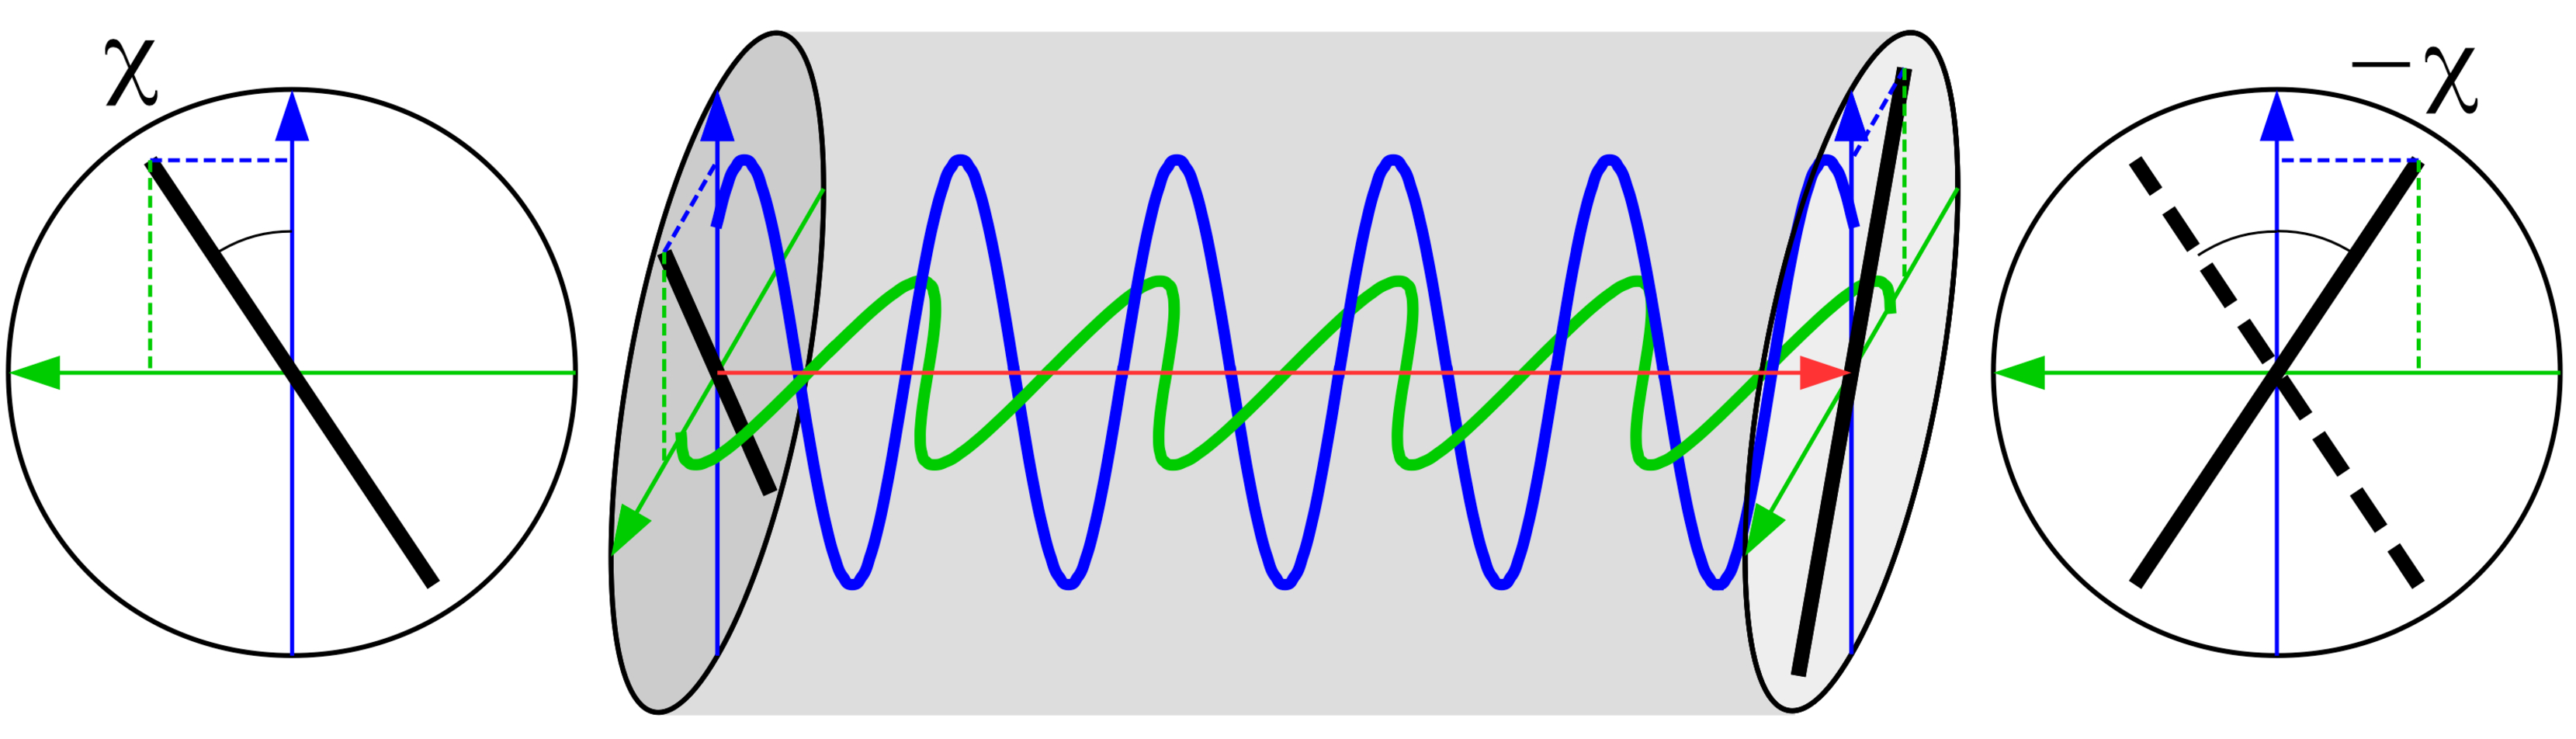
\includegraphics[width=0.8\textwidth]{simons_observatory/hwp_satoru.pdf}
    \caption{HWPを通過することで、偏光角が変化することを示した概念図。青い軸が1軸、緑の軸が2軸に対応する。
    入射した直線偏光の偏光角が1軸に対して $\chi$ であり、複屈折によって $-2\chi$ だけ変化する。}
    \label{fig:so-hwp_satoru}
\end{figure}

\section{偏光角較正の重要性とその手法}
\subsection{偏光角の誤較正に伴う偏光の漏れ込み}
CMB偏光観測実験でのBモード観測において、検出器の偏光角を精度よく知ることは極めて重要である。
その重要性を示すため、本項では偏光角の誤較正が観測されたBモード偏光にどのような影響を及ぼすかを考え、
SOにおいての要求偏光角較正精度を定める。

今、すべての検出器における偏光角を $\delta \theta$ だけ誤って較正してしまったとすると、
観測されるストークスパラメータ $Q_{\mathrm{obs}},\ U_{\mathrm{obs}}$ は真のストークスパラメータ $Q,\ U$ に対して
\begin{align}
    Q_{\mathrm{obs}} \pm iU_{\mathrm{obs}} &= e^{\pm i2\delta\theta}\qty(Q \pm iU) \\
    &= e^{\pm i2\delta\theta}\sum_{l=2}\sum_{m=-l}^{l} {}_{\pm 2}a_{lm}\ {}_{\pm 2}Y_{lm}(\theta, \phi)
\end{align}
と表される。\cite{so:Keeting_2023}\cite{so:Kaufman_2014}
Eモード、Bモード偏光を表現する係数 $a_{lm}^{E}, a_{lm}^{B}$ を用いると、
スピン2の球面調和関数で展開する際の係数 ${}_{\pm 2}a_{lm}$ は
\begin{equation}
    {}_{\pm 2}a_{lm} = -\qty(a_{lm}^{E} \pm i a_{lm}^{B})
\end{equation}
であるから
\begin{align}
    Q_{\mathrm{obs}} \pm iU_{\mathrm{obs}} &= \sum_{l=2}\sum_{m=-l}^{l} \qty[-\qty(a_{lm}^{E} \pm i a_{lm}^{B})]e^{\pm i2\delta\theta}\ {}_{\pm 2}Y_{lm}(\theta, \phi) \\
    &= \sum_{l=2}\sum_{m=-l}^{l} \qty[-\qty(a_{lm,\,\mathrm{obs}}^{E} \pm i a_{lm,\,\mathrm{obs}}^{B})] {}_{\pm2}Y_{lm}(\theta, \phi)
\end{align}
が観測されることとなる。したがって、パワースペクトル
\begin{equation}
    C_{l}^{XX'} = \dfrac{1}{2l+1}\sum_{m=-l}^{l}\left\langle \qty(a_{lm}^{X})^{*} a_{lm}^{X'} \right\rangle
\end{equation}
は、偏光角の誤較正によって
\begin{equation}
    \mqty( C_{\mathrm{obs},\,l}^{TT} \\[1ex]
           C_{\mathrm{obs},\,l}^{TE} \\[1ex]
           C_{\mathrm{obs},\,l}^{TB} \\[1ex]
           C_{\mathrm{obs},\,l}^{EE} \\[1ex]
           C_{\mathrm{obs},\,l}^{BB} \\[1ex]
           C_{\mathrm{obs},\,l}^{EB} )
    = \mqty( 1 & 0 & 0 & 0 & 0 & 0 \\[1ex]
             0 & \cos\qty(2\delta\theta) & 0 & -\sin\qty(2\delta\theta) & 0 & 0 \\[1ex]
             0 & \sin\qty(2\delta\theta) & 0 & \cos\qty(2\delta\theta) & 0 & 0 \\[1ex]
             0 & 0 & 0 & \cos^2\qty(2\delta\theta) & \sin^2\qty(2\delta\theta) & -\sin\qty(4\delta\theta) \\[1ex]
             0 & 0 & 0 & \sin^2\qty(2\delta\theta) & \cos^2\qty(2\delta\theta) & \sin(4\delta\theta) \\[1ex]
             0 & 0 & 0 & \sin\qty(4\delta\theta)/2 & -\sin\qty(4\delta\theta)/2 & \cos\qty(4\delta\theta)/2 )
    \mqty( C_{l}^{TT} \\[1ex]
              C_{l}^{TE} \\[1ex]
              C_{l}^{TB} \\[1ex]
              C_{l}^{EE} \\[1ex]
              C_{l}^{BB} \\[1ex]
              C_{l}^{EB} )
\end{equation}
となる。
標準宇宙モデルが正しく、原始密度ゆらぎがパリティ不変だった場合では $C_{l}^{TB}=C_{l}^{EB}=0$ であるが、
偏光角の誤較正は $C_{l}^{EE}$ から $C_{l}^{BB}$ への漏れ込みを引き起こす
\begin{equation}
    \label{eq:so-EtoBleakage}
    C_{\mathrm{obs},\,l}^{BB} = \sin^2\qty(2\delta\theta)C_{l}^{EE} + \cos^2\qty(2\delta\theta)C_{l}^{BB} .
\end{equation}

式\eqref{eq:so-EtoBleakage}に基づき、偏光角の誤較正が $C_{l}^{EE}$ から $C_{\mathrm{obs}, l}^{BB}$ への漏れ込みとして及ぼす影響を図\ref{}に示す。
誤較正の目安として、 $\delta\theta = 10, 1, 0.1\ \mathrm{deg}$ の場合をプロットした。

偏光角較正の要求精度は望遠鏡の感度やdelensingの能率、ノイズなどによって変化する。
SOにおいては、delensingの能率を 50\% とし、ノイズとして最も悲観的な場合を考えた場合においても、
$\delta\theta \leq 0.1\ \mathrm{deg}$ であればこの漏れ込みが生む $r$ への系統誤差は無視できるほどに小さくなる。\cite{so:Bryan_2018}
以上の理由から、SOでの偏光角較正の要求精度を $\delta\theta \leq 0.1\ \mathrm{deg}$ と定める。

\begin{figure}[H]
    \centering
    \caption{LAMBDA}を使って作成したEtoB leakageの図と、Lyth boundを示す図を載せる予定。
\end{figure}

\subsection{偏光角較正手法}
偏光角較正には、検出器間の相対的な偏光角を較正する相対角度較正と、
天球面上においてどの向きに偏光角を持っているかを較正する絶対角度較正が存在する。
本項では代表的な較正手法を紹介したのち、先行研究においてどのような手法をとり、その精度がどの程度であったかをまとめる。
\subsubsection{牡牛座かに星雲 (Tau A)}
Tau Aは強い直線偏光性を持つ光を放射する超新星残骸である。
その光の偏光角は観測周波数に依存している可能性が指摘されており、さらに高分解能望遠鏡による観測ではその構造が見えるため、偏光角を一意に決定することが難しいという課題がある。
また、偏光角は他の実験の観測結果にも依存しており、これらが潜在的な系統誤差として考慮される必要がある。
\subsubsection{月}
月はその表面で反射された光が月の中心から放射状に広がった偏光信号となる。
月の観測もTau Aと同じく構造による偏光角の違いが問題となり、ポインティング精度由来の系統誤差を生じる。
また、月は非常に明るいためTES検出器のダイナミックレンジを超えてしまい、SATでは観測が困難である。
\subsubsection{誘電体シート}
誘電体シートとは、膜状に張られたポリマーによって環境熱放射を反射させ、直線偏光を作り出す装置である。
その厚みを変えることで明るさの調整が容易であるが、望遠鏡の視野をすべて覆うためには装置が大型化する傾向にある。
また、周波数ごとに偏光特性が異なるため、較正に使用するためには高精度な周波数依存性の測定が必要である。

\subsubsection{デンスワイヤーグリッド}
デンスワイヤーグリッドは、金属ワイヤーを入射光に対して十分短い間隔で平行に張り巡らせた光学素子である。
近似的にはワイヤーが張られた方向に対しては電流を流すが、それに直行する方向には電流を流さない金属板として振る舞う。
そのため、入射光がワイヤーに沿った方向に偏光している場合には反射され、直行する方向に偏光している光は透過する。

デンスワイヤーグリッドは口径に対して平行に設置してしまうと検出器アレイとの間に多重反射が生じ、系統誤差を生じる。
これを抑制するため、デンスワイヤーグリッドを口径に対して傾けて設置する使用例が多い。
望遠鏡の口径を覆い、全検出器を同時に較正するためにはデンスワイヤーグリッド自体が大型化する必要があり、
作成する際にはワイヤー間隔を高精度に制御、長期間保つことが困難である。
また、デンスワイヤーグリッドはCMB観測実験で典型的な広い観測周波数帯で均一に偏光を生成することが難しいといった欠点も有する。

\subsubsection{スパースワイヤーグリッド}
スパースワイヤーグリッドは、金属ワイヤーを入射光に対して十分長い間隔で平行に張り巡らせた光学素子である。
原理は\ref{}にて後述するが、環境熱放射をワイヤーが反射することによりワイヤーに沿った方向に偏光した光を作り出す。

スパースワイヤーグリッドはワイヤー間隔が広いために多重反射を起こしにくく、望遠鏡の口径に対して平行に設置することができる。
そのため、デンスワイヤーグリッドよりも小型化が可能であり、製造難易度が比較的低い。
ワイヤー間隔が十分長いとみなせる範囲においては周波数依存性が小さいため、広い周波数帯で均一に偏光を生成することが可能である。
これらの特性から、複数の観測波長帯を持つすべての検出器を同時に較正することが可能であり、SOではスパースワイヤーグリッドを用いた偏光角較正装置が採用されている。

\subsubsection{自己較正}
標準宇宙モデルでは $C_{l}^{EB}=0$ である。
これを利用して、相対角度較正を十分に行なった上で $C_{l}^{EB} = 0$ とおくことで
$\delta\theta$ を求め、絶対角度較正を行う手法を自己較正と呼ぶ。
自己較正の精度は相対角度較正の精度と検出データ量に依存するため、検出器数が増大によって精度の向上が期待される。
しかし、$C_{l}^{EB}=0$ を仮定してしまうため、宇宙がパリティを破るような物理に対する感度を捨てることとなる。
そのため、これらの物理を探る上では自己較正以外の手法を用いて絶対角度較正を行うことが重要である。

\begin{table}
    \centering
    \caption{先行研究における偏光角較正手法とその精度の比較}
    \begin{tabular}{cccc}
        $\delta\theta$ & 観測周波数帯 [GHz] & 実験 & 較正手法 \\
        \hline
        \hline
        0.2 & 150 & POLARBEAR & 自己較正 \\
    \end{tabular}
    \label{tab:so-polarization_calibration}
\end{table}
\end{document}